\documentclass[12 pt]{article}
\usepackage[utf8]{inputenc}
\usepackage{amsmath}
\usepackage{amssymb,amsfonts,latexsym}
\usepackage{array}
\usepackage{bm}
\usepackage{float}
\usepackage{fancyhdr}
\usepackage{graphicx} 
\usepackage{longtable}
\usepackage{multicol}
\title{Bitacora Mecánica Clásica}
\date{Cristian Rafael Mendoza Maldonado\\ Mecánica Clásica\\Ubaldo Molina \\Física\\Univesidad del Atlántico\\2018-1}

\begin{document}
\maketitle


\section*{Ejericicio 1}
Hallar la divergencia en coordenadas esféricas:


\begin{figure}[H]
	\centering
	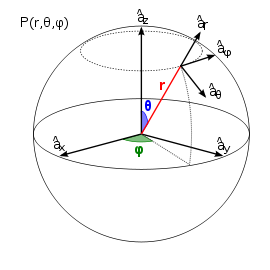
\includegraphics[scale= 0.6]{imagenes/a2.png}
	\caption{Coordenadas esféricas}
	\label{esfera}
\end{figure}


Bajos las tranformaciones descritas geométricamente por en la figura 1:
\begin{equation*}
x = r cos(\varphi) sin(\theta)  \hspace{0.5cm}
y = r sin (\varphi)sin(\theta) \hspace{0.5cm}
z = r cos(\theta)
\end{equation*}

La posición de una particula en coordenadas esféricas  esta descrita por: 

\begin{equation*}
\vec{r}= r cos(\varphi) sin(\theta)\hat{x}+ rsin (\varphi) sin(\theta) \hat{y} + r cos(\theta)\hat{z}
\end{equation*}

calculamos las derivadas direccionales 

\begin{equation*}
\frac{\partial \vec{r}}{\partial r} = cos(\varphi) sin (\theta) \hat{x} + 	sin (\varphi) sin(\theta) \hat{y} + cos(\theta)\hat{z}
\end{equation*}


\begin{equation*}
\frac{\partial \vec{r}}{\partial \varphi} =-r sin(\varphi)sin(\theta) \hat{x} + r cos(\varphi) sin(\theta
) \hat{y} + 0 \hat{z}
\end{equation*}


\begin{equation*}
\frac{\partial \vec{r}}{\partial \theta} = r cos(\varphi)cos(\theta) \hat{x}+r sin(\varphi)cos(\theta)\hat{y}-r sin(\theta)\hat{z}
\end{equation*}

Los factores de escala del sistema serian entonces:

\begin{equation*}
h_{r}= |\frac{\partial\vec{r}}{\partial r}| = 1\hspace{0.5cm} h_{\varphi}= |\frac{\partial\vec{r}}{\partial \varphi }| =r sin(\theta)\hspace{0.5 cm}h_{\theta}= |\frac{\partial\vec{r}}{\partial \theta}| = r
\end{equation*}

Partiendo de la defición de divergencia en coordenadas curvilineas, podemos calcularla en esféricas como una caso particular de las mismas:


\begin{equation*}
\nabla \cdot \vec{A} = \frac{1}{r^{2}sin(\theta)} \left[ \frac{\partial}{\partial r}(r^{2}sin(\theta) A_{r}) + \frac{\partial}{ \partial \theta} (rsin(\theta) A_{\theta}) + \frac{\partial}{\partial\varphi}  (r A_{\varphi}) \right]
\end{equation*}

\begin{equation*}
\nabla \cdot \vec{A} = \frac{1}{r^{2}sin(\theta)} \left[    2rsin(\theta)A_{r} + r^{2}sin(\theta) \frac{ \partial A_{r}}{\partial r}+ rsin(\theta) \frac{\partial A_{\theta}}{\partial \theta}+ rcos(\theta) A_{\theta} +  r \frac{\partial A_{\varphi}}{\partial \varphi}\right]
\end{equation*}


\begin{equation*}
\nabla \cdot \vec{A} = \frac{2 A_{r}}{r} + \frac{\partial A_{r}}{\partial r} + \frac{1}{r} \frac{\partial A_{\theta}}{\partial \theta} + \frac{1}{r tan(\theta)} A_{\theta} + \frac{1}{r sin(\theta)}  \frac{\partial A_{\varphi} }{\partial \varphi}
\end{equation*}


\section*{Ejericicio 2}
Dada la curva descrita por el vector posición:

\begin{equation*}
\vec{r} = Rcos(\omega t) \hat{x} + Rsin(\omega t)  \hat{y} + c t \hat{z} \hspace{1cm} (R,\omega, c) \hspace{0.5cm} constantes. 
\end{equation*}

Hallar $\hat{T},\hat{N}, \hat{\beta}$, k y $R_{c}$

\subsection*{Solución}
\begin{equation*}
\frac{d\vec{r}}{dt} = -R \omega sin(\omega t) \hat{x} + R \omega cos(\omega t)\hat{y} + c \hat{z} \hspace{1 cm}|\frac{d\vec{r}}{dt} |= \sqrt{(R\omega)^{2} +c^{2}}
\end{equation*}

\begin{equation*}
\hat{T} = \dfrac{\frac{d\vec{r}}{dt}}{|\frac{d\vec{r}}{dt}|} = \dfrac{-R \omega sin(\omega t) \hat{x} + R \omega cos(\omega t)\hat{y} + c \hat{z} }{\sqrt{(R\omega)^{2} +c^{2}}}
\end{equation*}


 calculando ahora 
 
\begin{equation*}
\frac{d\hat{T}}{dt} = \frac{-R \omega^{2} [cos(\omega t) \hat{x}+ sin(\omega t) \hat{y}]}{\sqrt{(R\omega)^{2} +c^{2}}} \hspace{1cm} |\frac{d\hat{T}}{dt}| = \frac{R \omega^{2}}{\sqrt{(R\omega)^{2} +c^{2}}}
\end{equation*}



La curvatura es entonces: 

\begin{equation*}
 k = \frac{1}{v}|\frac{d\hat{T}}{dt}| = \frac{1}{\sqrt{(R\omega)^{2} +c^{2}}} \frac{R \omega^{2}}{\sqrt{(R\omega)^{2} +c^{2}}}  =  \frac{R \omega^{2}}{(R\omega)^{2} +c^{2}}
\end{equation*}


y por tanto el radio de curvatura es:

\begin{equation*}
R_{c}= \frac{(R\omega)^{2} +c^{2}}{R \omega^{2}}
\end{equation*}

seguido a ello calculamos $\hat{N}$ como:

\begin{equation*}
\hat{N}= \frac{R_{c}}{v} \frac{d\hat{T}}{dt} = \dfrac{(R\omega)^{2} +c^{2}}{ (R\omega^{2})\sqrt{(R\omega)^{2} +c^{2}}}*\frac{-R \omega^{2} [cos(\omega t) \hat{x}+ sin(\omega t) \hat{y}]}{\sqrt{(R\omega)^{2} +c^{2}}} 
\end{equation*}

\begin{equation*}
\hat{N}= -[cos(\omega t) \hat{x}+ sin(\omega t) \hat{y}]
\end{equation*}

y finalmente 

\begin{equation*}
\hat{\beta} = \hat{T} X \hat{N} = [T_{y}N_{z}-T_{z}N_{y}]\hat{x} - [T_{x}N_{z}-T_{z}N_{x}] \hat{y}+[T_{x}N_{y}-T_{y}N_{x}]\hat{z}
\end{equation*}

sistemáticamente
\begin{equation*}
\beta_{x} = 0- \frac{c}{\sqrt{(R\omega)^{2} + c^{2}}}(-sin(\omega t)) \hspace{0.9cm}
\beta_{y}=  0- \frac{c}{\sqrt{(R\omega)^{2} + c^{2}}}(-cos(\omega t)) 
\end{equation*}

\begin{equation*}
\beta_{z}= \left[\frac{-R\omega sin(\omega t)}{\sqrt{(R\omega)^{2} + c^{2}}} (-sin(\omega t)) \right]-\left[\frac{-R\omega cos(\omega t)}{\sqrt{(R\omega)^{2} + c^{2}}}(-cos(\omega t))\right]
\end{equation*}

simplificando 

\begin{equation*}
\hat{\beta}= \frac{1}{\sqrt{(R\omega)^{2} + c^{2}}} \left[ c (sin(\omega t) \hat{x} + cos(\omega t )\hat{y}) -R\omega cos (2\omega t) \hat{z} \right]
\end{equation*}

\section*{Ejericicio 3} 
Hallar $\hat{r},\hat{\theta}, \hat{\phi}, \dot{\hat{r}}, \dot{\hat{\theta}}, \dot{\hat{\phi}}, \vec{v}, \vec{a}$ en coordenadas esféricas y relacionarlas.

\section*{Solución}

Normalizando las derivadas direccionales del ejercicio 1, logramos definir los vectores unitarios para el sistema esférico.

\begin{equation*}
\hat{r}= cos(\varphi) sin (\theta) \hat{x} + 	sin (\varphi) sin(\theta) \hat{y} + cos(\theta)\hat{z}
\end{equation*}

\begin{equation*}
\hat{\varphi}= -sin(\varphi)\hat{x} + cos(\varphi) \hat{y}
\end{equation*}

\begin{equation*}
\hat{\theta}=  cos(\varphi)cos(\theta) \hat{x}+ sin(\varphi)cos(\theta)\hat{y}- sin(\theta)\hat{z}
\end{equation*}

Calculando ahora las derivadas de dichos vectores:

\begin{equation*}
\dot{\hat{r}}_{(\varphi, \theta)} = \frac{\partial \hat{r}}{\partial \varphi} \dot{\varphi} + \frac{\partial \hat{r}}{\partial \theta}\dot{\theta}  = sin(\theta) (-sin(\varphi)\hat{x} + cos(\varphi) \hat{y})\dot{\varphi}
\end{equation*}

\begin{equation*}
+ (cos(\varphi)cos(\theta) \hat{x}+ sin(\varphi)cos(\theta)\hat{y}- sin(\theta)\hat{z}) \dot{\theta}
\end{equation*}



\begin{equation*}
\dot{\hat{\varphi}}_{(\varphi)} = \frac{\partial \hat{\varphi}}{\partial \varphi}\dot{\varphi}= (-cos(\varphi) \hat{x} -sin(\varphi) \hat{y}) \dot{\varphi}
\end{equation*}



 \begin{equation*}
 \dot{\hat{\theta}}_{\varphi, \theta} = \frac{\partial \hat{\theta}}{\partial \varphi}\dot{\varphi} + \frac{\partial \hat{\theta}}{\partial \theta} \dot{\theta}= (-sin(\varphi)cos(\theta)\hat{x} + cos(\varphi)cos(\theta) \hat{y}) \dot{\varphi}
   \end{equation*}

\begin{equation*}
+ (-cos(\varphi) sin (\theta) \hat{x} -	sin (\varphi) sin(\theta) \hat{y} - cos(\theta)\hat{z})\dot{\theta}
\end{equation*}


Relacionando cada derivada con las coordenadas unitarias del sistema llegamos a:


 \begin{equation*}
 \dot{\hat{r}} = sin(\theta)\dot{\varphi} \hat{\varphi} + \dot{\theta}\hat{\theta}
 \end{equation*}
 
 \begin{equation*}
 \dot{\hat{\varphi}}= - \dot{\varphi}\left( \hat{r} sin(\theta) +\hat{\theta}cos(\theta)  \right)
 \end{equation*}



\begin{equation*}
\dot{\hat{\theta}}= cos(\theta)\dot{\varphi}\hat{\varphi} - \dot{\theta} \hat{r}
\end{equation*}


Finalmente procedemos a calcular la velocidad y acelaración de dicha particula en este sistema de coordenadas:

Sea $\vec{r} = r \hat{r}$
\begin{equation*}
\dot{\vec{r}} = \dot{r} \hat{r} + r \dot{\hat{r}} = \dot{r} \hat{r} + r \left(sin(\theta)\dot{\varphi} \hat{\varphi} + \dot{\theta}\hat{\theta}\right)
\end{equation*}


\begin{equation*}
\ddot{\vec{r}} = \ddot{r}\hat{r} + \dot{r}\dot{\hat{r}} + \dot{r} \left(sin(\theta)\dot{\varphi} \hat{\varphi} + \dot{\theta}\hat{\theta}\right) + r \left(
cos(\theta)\dot{\theta}\dot{\varphi}\hat{\varphi} + sin(\theta)\ddot{\varphi}\hat{\varphi} + sin(\theta)\dot{\varphi}\dot{\hat{\varphi}} + \ddot{\theta}\hat{\theta}+ \dot{\theta}\dot{\hat{\theta}}\right)
\end{equation*}


sustituyendo las derivadas de los vectores unitarios y simplificando se llega a:

\begin{equation*}
\ddot{\vec{r}} = \ddot{r}\hat{r} + \dot{r} \left(sin(\theta)\dot{\varphi} \hat{\varphi} + \dot{\theta}\hat{\theta}\right) + \dot{r} \left(sin(\theta)\dot{\varphi} \hat{\varphi} + \dot{\theta}\hat{\theta}\right) + r (cos(\theta)\dot{\theta}\dot{\varphi}\hat{\varphi} + sin(\theta)\ddot{\varphi}\hat{\varphi}) 
\end{equation*}

\begin{equation*}
+ r sin(\theta)\dot{\varphi} \left( - \dot{\varphi}\left(\hat{r} sin(\theta) +\hat{\theta}cos(\theta)  \right) \right) + r\ddot{\theta} \hat{\theta}+ r\dot{\theta} \left(cos(\theta)\dot{\varphi}\hat{\varphi} - \dot{\theta} \hat{r}\right)
\end{equation*}



Reagrupando términos:

 \begin{equation*}
 \ddot{\vec{r}} =  \left( \ddot{r} - r \dot{\varphi}^{2} sin^{2}(\theta) -  r \dot{\theta}^{2} \right) \hat{r} 
 + \left(2 \dot{r}\dot{\varphi}sin(\theta)+ 2 r \dot{\theta}\dot{\varphi}cos(\theta) + r \ddot{\varphi} sin(\theta)\right) \hat{\theta} 
 \end{equation*}

 \begin{equation*}
 +\left(  2 \dot{r}\dot{\theta} + r \ddot{\theta} - r \dot{\varphi}^{2} cos(\theta)sin(\theta) \right) \hat{\varphi} 
 \end{equation*}



\section*{Ejericicio 4}
Desarrolla la maquina de Atwood usando las leyes de Newton, y luego por medio de las ecuaciones de lagrange.


\subsection*{Solución}
Recordando: La máquina de Atwood consiste en dos masas, $ m_{1}$ y  $m_{2}$ , conectadas por una cuerda inelástica de masa despreciable con una polea ideal de masa despreciable.


Desarrollamos como primera parte usando las ecuaciones de newton. 

\begin{figure}[H]
	\centering
	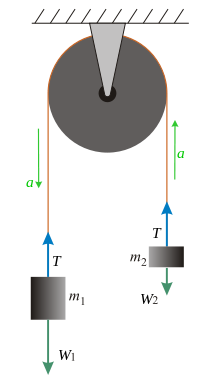
\includegraphics[scale= 0.5]{imagenes/a1.png}
	\caption{Maquina de atwood}
	\label{atwood}
\end{figure}


planteando los diagramas de cuerpo libre para los cuerpos 1 y 2. En donde $m_{1} >m_{2}$.



%adjuntar diagramas de cuerpo libre de cada masa.

\begin{equation}
\sum F_{y}^{1}= T-m_{1}g =- m_{1}a 
\end{equation}

\begin{equation}
\sum F_{y}^{2}= T-m_{2}g = m_{2}a 
\end{equation}


Restando (2)-(1), llegamos a:

\begin{equation*}
[m_{1} - m_{2}]g = [m_{1} + m_{2}] a
\end{equation*}


\begin{equation}
a = \frac{m_{1} - m_{2}}{m_{1} + m_{2}} g
\end{equation}


sustiendo en (1) llegamos a que: 

$$ T = \frac{2m_{1}m_{2}}{m_{1}+m_{2}}g $$



Sea l la longitud de la cuerda y x la altura de la masa 1 medida desde el punto más alto que alcanza la cuerda, las energias del sistema estarian descritas como sigue:

\begin{equation*}
K = \frac{1}{2} (m_{1}+m_{2}) (\dot{x})^{2} \hspace{0.5cm} U= -m_{1}gx-m_{2}g(l-x)
\end{equation*}

Cuyo lagrangiano es


\begin{equation*}
L = K-U = \frac{1}{2} (m_{1}+m_{2}) (\dot{x})^{2} +m_{1}gx +m_{2}g(l-x)
\end{equation*}

Y cuya unica ecuación de euler-lagrange es

\begin{equation*}
\frac{\partial L}{\partial x} - \frac{d}{dt} \left( \frac{\partial L}{\partial \dot{x}}\right) = 0
\end{equation*}

\begin{equation*}
(m_{1}-m_{2})g - (m_{1}+m_{2}) \ddot{x}= 0
\end{equation*}

Esto es
\begin{equation*}
\ddot{x}= \dfrac{(m_{1}-m_{2})}{(m_{1}+m_{2})} g
\end{equation*}

Puesto el sistema maneja una aceleración constante, podemos hallar la ecuación del movimiento desde la cinemática como sigue:

$$ y_{t}= y_{0}+v_{yo}t+\frac{1}{2}at^{2} $$

\section*{Ejericicio 5}
Un esféra de masa $m_{1}$ y radio R se sujeta a una barra rigida de  masa $m_{2}$ y longitud 2L. El sistema se suspende sobre un punto a, el cual puede moverse en el eje x.
Suponiendo que $\theta$ es el ángulo que hace el pendulo con el eje vertical.

\begin{enumerate}
	\item Hallar el lagrangiano del sistema.
	\item Las ecuaciones de Euler-lagrange.
\end{enumerate}



\subsection*{Solución}

1. Inicialmente calculamos el centro de masas del sistema:

\begin{equation*}
r_{cm}= \dfrac{L m_{1} + (2L + R)m_{2}}{m_{1}+m_{2}} =h
\end{equation*}

Siendo valida las transformaciones


\begin{equation*}
X = x + h sin(\theta) \hspace{0.5cm} Y= -h cos(\theta)
\end{equation*}

\begin{equation*}
\dot{X}= \dot{x} + h \dot{\theta}cos(\theta) \hspace{0.5cm} \dot{Y}= h \dot{\theta}sin(\theta)
\end{equation*}

Por simplicidad consideremos tambien $ M = m_{1} + m_{2}$. y por el teorema de steiner tenemos que: 

\begin{equation*}
I = I_{varilla} + I_{esfera} = \frac{m_{1}L^{2}}{3} + \frac{2m_{2} R^{2}}{5} + m_{2} (L+R)^{2} 
\end{equation*}


Ahora las energias del sistema quedan expresadas por:

\begin{equation*}
K = \frac{1}{2} M (\dot{X}^{2} + \dot{Y}^{2}) + \frac{1}{2}I \dot{\theta}^{2} \hspace{0.5cm} U= -MgLcos(\theta)
\end{equation*}


\begin{equation*}
L = K- U = \frac{1}{2} M \left[\dot{x}^{2}+ 2\dot{x}h\dot{\theta}cos(\theta)+(h\dot{\theta}cos(\theta))^{2}\right] + \frac{1}{2} I \dot{\theta}^{2} + gML cos(\theta)
\end{equation*}


2. Ahora calculando las ecuaciones de euler lagrange para este sistema tenemos:


para $q_{1} = x$
\begin{equation*}
\frac{\partial L }{\partial x} - \frac{d}{dt} \left( \frac{\partial L}{\partial \dot{x}}\right)= 0
\end{equation*}

\begin{equation*}
 0 - \frac{d}{dt}M \left( \dot{x} + \dot{\theta}h cos(\theta)\right) = 0 
\end{equation*}
 Esto es: 
 
 
 \begin{equation*}
 P_{x} = \dot{x} + \dot{\theta}h cos(\theta)
 \end{equation*}
 
 derivando tenemos que:
 
 \begin{equation*}
  \ddot{x} + \ddot{\theta}h cos(\theta) - \dot{\theta}^{2} hsin(\theta)=0
 \end{equation*}


Para $q_{2}= \theta$

\begin{equation*}
\frac{\partial L }{\partial \theta} - \frac{d}{dt} \left( \frac{\partial L}{\partial \dot{\theta}}\right)= 0
\end{equation*}

\begin{equation*}
-\dot{x}h\dot{\theta}sin(\theta) - h\dot{\theta}cos(\theta)sin(\theta)- gMLsin(\theta)-\frac{d}{dt} \left( \dot{x}hcos(\theta)+\dot{\theta} h^{2} cos^{2}(\theta)\right) = 0 
\end{equation*}



\begin{equation*}
-\dot{x}h\dot{\theta}sin(\theta) - h\dot{\theta}cos(\theta)sin(\theta)- gMLsin(\theta)-
\end{equation*}

\begin{equation*}
\left(
\ddot{x}h\cos(\theta)+ \ddot{\theta}h^{2} cos^{2}(\theta) -2h^{2}cos(\theta)sin(\theta)\dot{\theta}^{2}- \dot{x} h sin(\theta) \dot{\theta} \right)= 0
\end{equation*}


simplificando tenemos que:


\begin{equation*}
-h\dot{\theta}cos(\theta)sin(\theta)- gML sin(\theta) - \ddot{x}h cos(\theta)-\ddot{\theta}h^{2}cos^{2}(\theta)+2h^{2} cos(\theta)sin(\theta)\dot{\theta}^{2} = 0
\end{equation*} 

 
 \begin{equation*}
 -h\dot{\theta}cos(\theta)sin(\theta)- gML sin(\theta) - hcos(\theta) \left( (\ddot{x} + \ddot{\theta}h cos(\theta) - \dot{\theta}^{2} hsin(\theta)) - \dot{\theta}^{2} hsin(\theta)\right) = 0 
 \end{equation*}
 sustituyendo la ecuación de X finalmente llegamos a:
\begin{equation*}
hcos(\theta) \left(\dot{\theta}^{2} - \dot{\theta} \right)- gML = 0
\end{equation*}

o lo que es lo mismo: 


\begin{equation*}
\dot{\theta} = \dfrac{1+- \sqrt{1-\frac{4gML}{h cos(\theta)}}}{2} = \omega_{1,2}
\end{equation*}



Sustituyendo $\theta$ en $P_{x}$, llegamos a: 

\begin{equation*}
\dot{x} = P_{x} - h cos(\theta) \left(\dfrac{1+- \sqrt{1-\frac{4gML}{h cos(\theta)}}}{2} \right) = P_{x} - \frac{hcos(\theta)}{2} -+ \sqrt{\left( \frac{hcos(\theta)}{2}\right) ^{2} - gML}  = v_{x}
\end{equation*}

integrando $\dot{\theta}$ y $\dot{x}$ llegamos a las funciones de movimiento del sistema, las cuales son:

\begin{equation*}
x = v_{x} t \hspace{0.5 cm} \theta = \omega_{1,2} t
\end{equation*}


\section*{Ejericicio 6}
Llegar a las ecuaciones diferenciales del potencial de keppler via hamilton.

\subsection*{Solución}

Sea el vector velocidad en coordenadas esféricas
\begin{equation*}
\dot{\vec{r}} = \dot{r} \hat{r} + r \dot{\hat{r}} = \dot{r} \hat{r} + r \left(sin(\theta)\dot{\varphi} \hat{\varphi} + \dot{\theta}\hat{\theta}\right)
\end{equation*}
las energias vendrian dadas por:


\begin{equation*}
K = \frac{1}{2} m \left( \dot{r}^{2} + r^{2}\dot{\theta}^{2} + r^{2}\dot{\varphi}^{2}sin^{2}(\theta)  \right) \hspace{0.5 cm} U= \frac{k}{r}
\end{equation*}


cuyo lagrangiano seria:

\begin{equation*}
L =  \frac{1}{2} m \left( \dot{r}^{2} + r^{2}\dot{\theta}^{2} + r^{2}\dot{\varphi}^{2}sin^{2}(\theta)\right)  -\frac{k}{r}
\end{equation*}


Los momentos generalizados vendrian dados por:


\begin{equation*}
p_{r}= \frac{\partial L }{\partial r} =m \dot{r}  \hspace{0.5cm} \dot{r} = \frac{P_{r}}{m}
\end{equation*}

\begin{equation*}
p_{\theta}= \frac{\partial L }{\partial \theta} =	mr^{2} \dot{\theta}  \hspace{0.5cm} \dot{\theta} =\frac{P_{\theta}}{m r^{2}}
\end{equation*}


\begin{equation*}
p_{\varphi}= \frac{\partial L }{\partial \varphi}= m r^{2}sin^{2}(\theta) \dot{\varphi}  \hspace{0.5cm} \dot{\varphi}= \frac{P_{\varphi}}{m r^{2}sin^{2}(\theta)}
\end{equation*}


De manera que el Hamiltoniano quedaria expresado por:

\begin{equation*}
H = \sum_{i=1}^{3} \dot{q_{i}} p_{i} - L = \dot{r}P_{r} +\dot{\theta} p_{\theta} +   \dot{\varphi} p_{\varphi} -\left(\frac{1}{2} m \left( \dot{r}^{2} + r^{2}\dot{\theta}^{2} + r^{2}\dot{\varphi}^{2}sin^{2}(\theta)\right)  -\frac{k}{r} \right) 
\end{equation*}

\begin{equation*}
H = \frac{p_{r}^{2}}{m} + \frac{p_{\theta}^{2}}{mr^{2}} +\frac{p_{\varphi}^{2}}{mr^{2}sin^{2}(\theta)}- \frac{p_{r}^{2}}{2m} - \frac{p_{\theta}^{2}}{2mr^{2}}-\frac{p_{\varphi}^{2}}{2mr^{2}sin^{2}(\theta)}+ \frac{k}{r}
\end{equation*}

\begin{equation*}
= \frac{p_{r}^{2}}{2m} + \frac{p_{\theta}^{2}}{2mr^{2}}+\frac{p_{\varphi}^{2}}{2mr^{2}sin^{2}(\theta)}+ \frac{k}{r}
\end{equation*}


Calculando ahora las ecuaciones de hamilton:


Para $q_{1} = r$

\begin{equation*}
\dot{r}= \frac{\partial H}{\partial p_{r}} = \frac{P_{r}}{m} \hspace{0.5cm} \rightarrow \dot{p_{r}} = m \ddot{r}
\end{equation*}

\begin{equation*}
\dot{P_{r}} = - \frac{\partial H}{\partial r}= \frac{P_{\theta}^{2}}{m r^{3}} + \frac{P_{\varphi}^{2}}{m r^{3} sin^{2}(\theta)} + \frac{k}{r^{2}} = m \ddot{r}
\end{equation*}


\begin{equation*}
\ddot{r} = 	r\dot{\theta}^{2} + \dot{\varphi}^{2} r sin(\theta) + \frac{k}{m r^{2}}
\end{equation*}


Para $q_{2}= \theta$

\begin{equation*}
\dot{\theta} = \frac{\partial H }{ \partial p_{\theta}} = \frac{p_{\theta}}{mr^{2}} \hspace{0.5cm}\rightarrow \dot{p_{\theta}}= m(r\dot{r}\dot{\theta}+ r^{2}\ddot{\theta})
\end{equation*}

\begin{equation*}
\dot{p_{\theta}} = - \frac{\partial H}{\partial \theta} = \frac{p_{\varphi}^{2}cos(\theta)}{mr^{2}sin^{3}(\theta)} = m(r\dot{r}\dot{\theta}+ r^{2}\ddot{\theta})
\end{equation*}

reemplazando $p_{\varphi}$

\begin{equation*}
\ddot{\theta} = \dfrac{r sin(\theta)cos(\theta)\dot{\varphi}^{2}- 2 \dot{r}\dot{\theta}}{r}
\end{equation*}


Para $q_{3} = \varphi$


\begin{equation*}
\dot{\varphi}= \frac{\partial H }{ \partial p_{\varphi}}= \frac{p_{\varphi}}{mr^{2}sin^{2}(\theta)} \hspace{0.5cm} \rightarrow p_{\varphi} = \dot{\varphi}mr^{2}sin^{2}(\theta)
\end{equation*}

 \begin{equation*}
 \dot{p_{\varphi}} = -\frac{\partial H }{ \partial \varphi}= 0 
 \end{equation*}

\begin{equation*}
p_{\varphi} = cte = \dot{\varphi}mr^{2}sin^{2}(\theta)
\end{equation*}


\section*{Ejericicio 7}
Probar una ley de keppler.

\subsection*{Solución}
Escojemos la primera ley y partimos del mismo potencial del ejercicio anterior.

\begin{equation*}
U = \frac{k}{r}
\end{equation*}
Considerando ahora la fuerza que siente una particula de masa m producto de este potencial

\begin{equation*}
F_{r} = -\frac{\partial U }{\partial r} = \frac{k}{r^{2}} \hat{r}
\end{equation*}


Sustituyendo en la ecuación de una orbita bajo fuerzas centrales: 


\begin{equation*}
\frac{d^{2}u}{d\theta} + u = -\frac{km}{l^{2}}  \hspace{0.5 cm}  ; u = \frac{1}{r}
\end{equation*}


el lado derecho de la ecuación se comvierte en una constante para potenciales de esta forma. Esta ecuación puede integrarase para dar:

\begin{equation*}
u = \frac{1}{r}= -\frac{km}{l^{2}} \left( 1 - e cos(\theta -\theta_{o}) \right) 
\end{equation*}

donde e y $\theta_{o}$ son constantes de integración, esta última representa la orienteación de la curva además el  lazo de la curva depende de la constante e, siendo esta última ecuación la de una sección cónica.


Una sección cónica es el lugar de un punto cuya distancia desde un punto dado, el foco, tiene una relación constante a su distancia desde una línea dada, la directriz. La relación es e, la excentricidad de la cónica. El foco se toma como el origen, y la directriz está a una distancia s a la izquierda del foco. Entonces nosotros tenemos

\begin{equation*}
r = e(s +r cos(\theta)) \hspace{0.5cm} u = \frac{1}{r}= \frac{1}{es}(1- e cos(\theta))
\end{equation*}


La segunda ecuacion es similar a la que se encontro para el movimiento de una particula bajo este tipo de potencial.En un potencial de tipo atractivo como son los gravitacionales, k toma valores negativos.


Además, como $u >0$ porque r tambien lo es


\begin{equation*}
\frac{km}{l^{2}} -\frac{km}{l^{2}} e cos(\theta) \eqslantgtr 0
\end{equation*}
\begin{equation*}
-\frac{km}{l^{2}}e cos(\theta)\eqslantgtr \frac{km}{l^{2}}
\end{equation*}




Por lo cual $e \eqslantless 1$ en donde  u nunca tiende a 0 y r permanece finita. Para el caso de $e=1$ se trata de una parabola, y para más común en orbitas planetarias $e<1$, la curva es una elipse.



















\section*{Ejericicio 8}
Probar que el intervalo espacio-tiempo es invariante mediante las transformaciones de lorenzt.
 $(\Delta S ^{'})^{2} = (\Delta S^{'})^{2}$


\subsection*{Solución}
En donde $ (\Delta S^{'})^{2} =  c^{2}(\Delta t^{'})^{2} - (\Delta x^{'})^{2}$
Una vez aplicada las transformaciones de lorentz:

\begin{equation*}
 \Delta x ^{'}= \gamma (\Delta x - v \Delta t) \hspace{0.5cm} \Delta t^{'}= \gamma(\Delta t - \frac{v}{c^{2}}\Delta x)
\end{equation*}



\begin{equation*}
(\Delta S^{'})^{2} = c^{2} \gamma^{2} \left((\Delta t)^{2} - 2 (\Delta x)(\Delta t) \frac{v}{c^{2}} + \frac{v^{2}}{c^{4}} (\Delta x)^{2} \right) - \gamma^{2} \left( (\Delta x)^{2} - 2 (\Delta x)(\Delta t)v + v^ {2}(\Delta x)^{2} \right) 
\end{equation*}



Reagrupando y cancelando términos semejantes

\begin{equation*}
(\Delta S^{'})^{2} = (\Delta t)^{2} \left(  c^{2} \gamma^{2}- \gamma^{2} v^{2}\right) - (\Delta x)^{2} \left( \gamma^{2} - \gamma^{2}\frac{v^{2}}{c^{2}}  \right)  = \left( c^{2} (\Delta t)^{2} - (\Delta x)^{2}\right)  \gamma^{2} \left( 1 - \frac{v^{2}}{c^{2}}  \right) 
\end{equation*}


En donde $\gamma^{2} \left( 1 - \frac{v^{2}}{c^{2}}  \right)  = 1 $


\begin{equation*}
(\Delta S^{'})^{2} =\left( c^{2} (\Delta t)^{2} - (\Delta x)^{2}\right)  = (\Delta S)^{2}
\end{equation*}


Extrapolando el mismo procedimiento a tres dimensiones espaciales

\begin{equation*}
(\Delta S^{'})^{2} = c^{2} (\Delta t)^{2} - (\Delta x)^{2} - (\Delta y)^{2}- (\Delta z)^{2} = (\Delta S)^{2}
\end{equation*}


Probando así la invarianza del intervalo espacio-tiempo bajo las transformaciones de lorentz.


\section*{Ejericicio 9}
Realize las transformaciones de energía y momento.



\section*{Ejericicio 10}
Hallar la matriz de inercia de un paralepipedo recto de masa M de lados a,b,c. Densidad volumétrica $\rho =\frac{M}{abc}$; dm = $\rho$ dv.


\subsection*{Solución}
 
\begin{figure}[H]
	\centering
	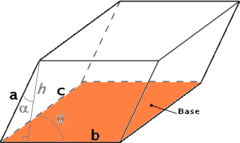
\includegraphics[scale= 0.6]{imagenes/a3.png}
	\caption{paralelepipedo oblicuo}
	\label{parelelepipedo}
\end{figure}


De la figura vemos que las dimensiones del paralelepipedo van en cada eje respectivamente:


\begin{equation*}
x = [0,a] \hspace{0.5cm} y= [0, b* sin(\theta)] \hspace{0.5cm} z= [0, c*sin(\alpha)]
\end{equation*}

calculamos los momentos de inercia:


\begin{equation*}
I_{xx}=\int_{0}^{a}\int_{0}^{csin(\alpha)}\int_{0}^{bsin(\theta)} (y^{2} + z^{2})\rho dydzdx = \rho a sin(\alpha) sin(\theta) \left[ \frac{1}{3}b^{3}csin^{2}(\theta) + \frac{1}{3}c^{3}b sin^{2}(\alpha)\right]
\end{equation*}


\begin{equation*}
I_{xx}= \frac{1}{3}Msin(\alpha) sin(\theta) \left
[b^{2}sin^{2}(\theta) + c^{2} sin(\alpha)\right]
\end{equation*}


\begin{equation*}
I_{yy}=\int_{0}^{bsin(\theta)}\int_{0}^{csin(\alpha)}\int_{0}^{a} (x^{2} + z^{2})\rho dxdzdy = \rho b sin(\theta) \left[\frac{a^{3}}{3} b sin(\alpha) + \frac{c^{3}}{3}asin^{3}(\alpha)\right]
\end{equation*}


\begin{equation*}
I_{yy}= \frac{1}{3}M sin(\alpha)sin(\theta) \left[a^{2} + c^{2}sin^{2}(\alpha) \right]
\end{equation*}


\begin{equation*}
I_{zz}=\int_{0}^{csin(\alpha)}\int_{0}^{bsin(\theta)}\int_{0}^{a} (x^{2} + y^{2})\rho dxdydz = \rho c sin(\alpha) \left[ \frac{a^{3}}{3} b sin(\theta) + \frac{b^{3}}{3}asin^{3}(\theta)\right]
\end{equation*}

\begin{equation*}
I_{zz}= \frac{1}{3}M sin(\alpha)sin(\theta) \left[a^{2} + b^{2}sin^{2}(\theta) \right]
\end{equation*}

\begin{equation*}
I_{xy} = \int_{0}^{csin(\alpha)} \int_{0}^{bsin(\theta)} \int_{0}^{a} xy \rho dx dy dz = \frac{1}{4}\rho a^{2} b^{2}sin^{2}(\theta) c sin(\alpha)   
\end{equation*}


\begin{equation*}
I_{xy} = \frac{1}{3} M sin(\alpha)sin(\theta) \left[ ab sin(\theta) \right]
\end{equation*}


\begin{equation*}
I_{xz} =  \int_{0}^{bsin(\theta)}\int_{0}^{csin(\alpha)}  \int_{0}^{a} xz \rho dx  dz dy = \frac{1}{4}\rho a^{2} c^{2} sin^{2}(\alpha) b sin(\theta)
\end{equation*}

\begin{equation*}
I_{xz} =  \frac{1}{3}M sin(\alpha)sin(\theta) \left[ ac sin(\alpha)\right]
\end{equation*}

\begin{equation*}
I_{yz} = \int_{0}^{a} \int_{0}^{csin(\alpha)} \int_{0}^{bsin(\theta)}  yz \rho  dy dz dx = \rho b^{2} sin^{2}(\theta) c^{2}sin^{2}(\alpha) a 
\end{equation*}

\begin{equation*}
I_{yz}= \frac{1}{3}M sin(\alpha)sin(\theta) \left[ bc sin(\alpha) sin(\theta)\right]
\end{equation*}

I= $ \frac{1}{3}M sin(\alpha)sin(\theta)$

\[
\begin{bmatrix}
b^{2}sin^{2}(\theta) + c^{2} sin(\alpha)& ab sin(\theta)& ac sin(\alpha)\\
ab sin(\theta)&a^{2} + c^{2}sin^{2}(\alpha) &  bc sin(\alpha) sin(\theta)\\
ac sin(\alpha)& bc sin(\alpha) sin(\theta) &a^{2} + b^{2}sin^{2}(\theta)\\
\end{bmatrix}
\]


\end{document}
